\subsection{RabbitMQ}
RabbitMQ ist eine von Pivotal Software entwickelte Message Oriented Middleware,
welche das AMQP Protokoll implementiert. Der Server ist in Erlang geschrieben und
plattformunabhängig. Er unterstützt die in \ref{compability:table} dargestellten
Programmiersprachen. Nicht nur AMQP, sondern auch eine Reihe weiterer Protokolle,
wie etwa das im IoT-Umfeld beliebte MQTT, werden unterstützt \cite{dobbelaere2017kafka}.
Daher eignet sich RabbitMQ besonders in Bereichen, in denen mehrere Protokolle zum
Einsatz kommen, oder AMQP eine harte Anforderung ist.

RabbitMQ verwendet eine Queue. Im Detail werden Nachrichten vom Producer an eine
sogenannte Exchange, welche als Router für Nachrichten fungiert, gesendet.
Diese Exchange entscheidet, an welche Queue die Nachricht weitergeleitet wird.
Dabei basiert die Entscheidung auf vorhandenen Routingregeln. Danach wird die
Nachricht in der Queue solange zwischengespeichert, bis sie zugestellt werden
kann. Anders als bei RabbitMQ werden bereits zugestellte Nachrichten daraufhin
gelöscht. \cite{RabbitMQ:online}

\paragraph{Routing}
Da RabbitMQ AMQP implementiert, können sehr komplexe Routing-Logiken umgesetzt
werden. Dabei ist hauptsächlich Topic-basiertes Routing relevant, da dies leichter mit dem
Routing von Kafka verglichen werden kann.
Hierbei wird ein sogenanntes Multipart-Routing unterstützt: Die Nachrichten
werden mit Topics in der Form \texttt{a.b.c} versehen, welche dann mithilfe
von Wildcards gefiltert werden können. Die Konfigurationsmöglichkeiten sind
hierbei sehr vielfältig. Ferner existiert auch ein inhaltsbasiertes Routing. \cite{RabbitMQ:online}

\paragraph{Besonderheiten}
\begin{figure}
  \centering
  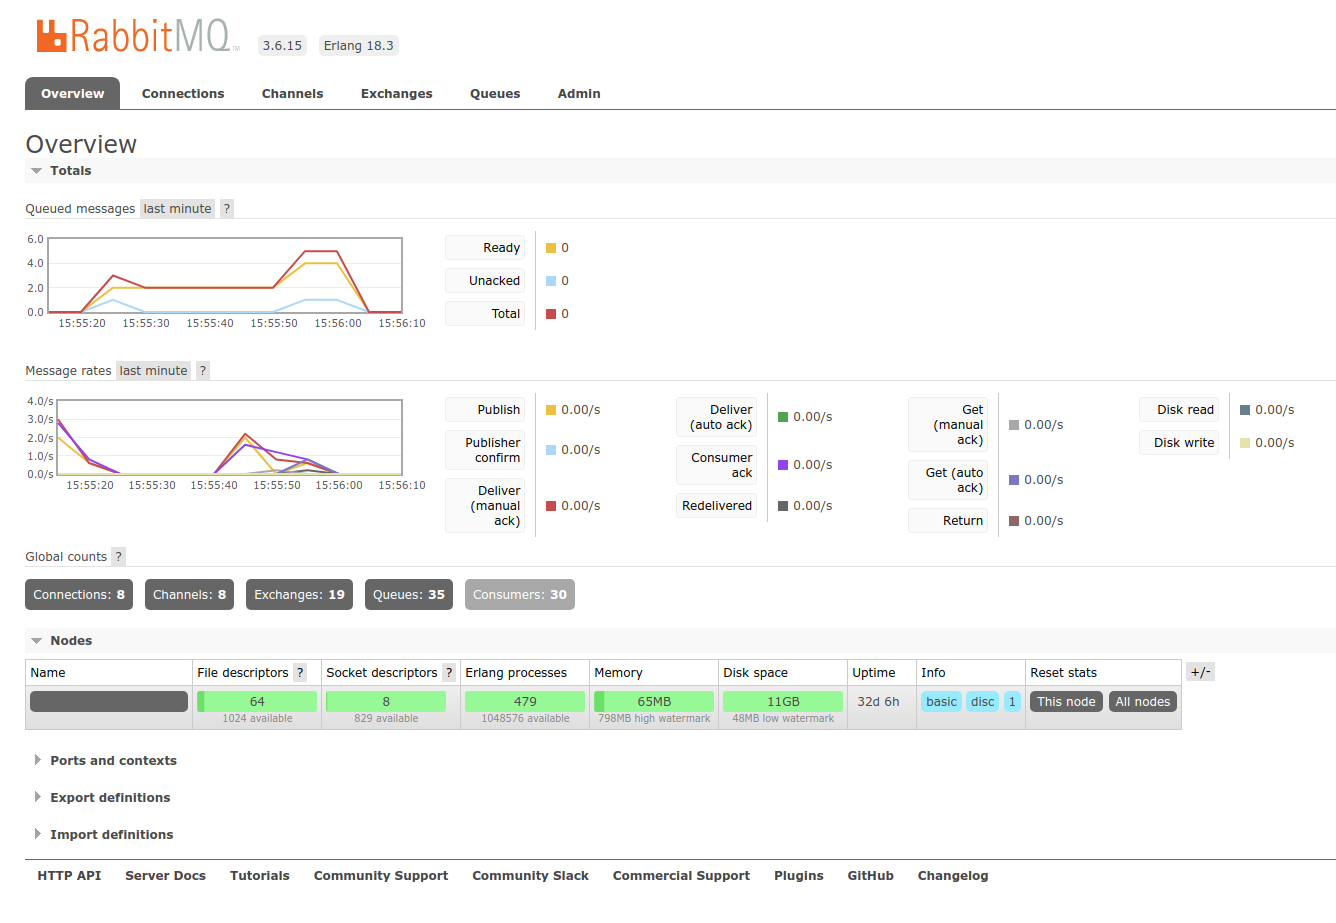
\includegraphics[width=.9\textwidth]{figures/rabbitmq.png}
  \caption{Weboberfläche von RabbitMQ}
  \label{rabbitmq:webinterface}
\end{figure}
RabbitMQ ist von Haus aus mit sehr umfangreichen Monitoring und Management Tools
ausgestattet. Diese erlauben, die meisten wichtigen Aspekte auf einen Blick
zu kontrollieren. In Darstellung \ref{rabbitmq:webinterface} sieht man die Weboberfläche einer RabbitMQ
Instanz, die aktiv verwendet wird. Dabei sind Statistiken zur Gesamtlast sichtbar.
Ferner kann RabbitMQ bei Bedarf komplett in-memory, also ohne Nachrichten auf
einer Festplatte zwischenzuspeichern, sondern nur im Arbeitsspeicher, betrieben
werden.

Die Consumer werden von RabbitMQ aktiv protokolliert. So besteht stets
Transparenz, welcher Consumer welche Nachrichten bereits empfangen hat.
Außerdem können Nachrichten pro Queue mit einer Time to Live, also einer
Gesamtdauer, die eine Nachricht im System existieren darf, versehen werden. Dies
macht vor allem im Kontext von Echtzeit-Daten Sinn.

Auch unterstützt RabbitMQ direkte Antworten auf Nachrichten. Bei Bedarf kann auf
eine Nachricht direkt und ohne entsprechende Antwortqueues geantwortet werden.

\paragraph{Analyse nach Eigenschaftenkatalog}
Die von RabbitMQ übernommenen Garantien bezüglich der Zustellung von Nachrichten sind,
wie auch bei Kafka, \textbf{at least once}. Es besteht also Risiko, dass Nachrichten
doppelt gesendet werden, jedoch nicht, dass sie nie gesendet werden.

Anders verhält es sich bei der Sortierung. RabbitMQ unterstützt \textbf{global order}. Die Exchange
übergibt einer Queue stets die Nachrichten in Batches, die vorsortiert sind.
Verliert ein Client also eine Message aus einer Batch, stellt dies RabbitMQ fest,
und kann die einzelne Nachricht erneut senden.
Das Routing kann, wie bereits erwähnt, sehr komplex sein, und es werden neben
Topic basiertem Routing noch weitere Arten unterstützt.

RabbitMQ unterstützt High Availability durch Replikation vollständiger Ex\-changes.
Allerdings ist der damit verbundene Konfigurationsaufwand im Vergleich zu Kafka
erheblich. Ferner kann relativ einfach skaliert werden, indem dem Cluster neue
Instanzen zugefügt werden. Dabei können neue Queues auf der neuen Instanz zum
Master werden, das heißt, die andere Instanz kopiert sie zwar, aber Consumer
verwenden bevorzugt diesen Master. Anders als bei Kafka kann jedoch keine
bereits bestehende Queue eine neue Instanz zu Ihrem Master machen. Somit ist die
Skalierung mit mehr Aufwand als bei Kafka verbunden.
\paragraph{Use Cases}
Aufgrund der beschriebenen Besonderheiten RabbitMQs eignet sich dieses hervorragend
für Anwendungen, die keine extremen Datenmengen verarbeiten müssen. Dank des
sehr fortgeschrittenen Routings von AMQP können leicht Anwendungen mit sehr
vielen Clients bedient werden.

Ein idealer Use Case ist beispielsweise IoT. Sowohl im privaten, wie im
industriellen Umfeld, kann von geringen Latenzen und dem Support des MQTT
Protokolls profitiert werden. Des Weiteren trägt ein fortgeschrittenes
Monitoring zum einfachen Debuggen von Anwendungen bei.
Auch wird RabbitMQ häufig im Enterprise Bereich eingesetzt. Durch die
Unterstützung von mehreren standardisierten Protokollen wird eine Integration in
ein Umfeld mit stark heterogenen Teilnehmern und auch die Anbindung von älteren
Systemen an RabbitMQ begünstigt.

\newpage
\subsection{NSQ}
NSQ ist eine relativ neue Implementierung des Unternehmens bitly, die ähnliche
Möglichkeiten wie eine MOM bietet. Dabei entfällt jedoch eine zentrale Instanz.
Das bedeutet, es gibt keinen Server, mit dem alle Kommunikationspartner verbunden
sind, sondern alle Teilnehmer sind untereinander verbunden.
Damit man diese Verbindungen nicht
verwalten muss, gibt es eine \textit{Service Discovery}. Diese kann andere
Instanzen entdecken und stellt so ein Netzwerk her. Dezentrale Lösungen wie
diese existierten jedoch schon vor NSQ, beispielsweise ZeroMQ.
Der Client sowie die Service Discovery von NSQ sind in Go implementiert. \cite{NSQ:online}

\paragraph{Besonderheiten}
Wie bereits erwähnt, entfällt eine zentrale Instanz, über die die Nachrichten
geleitet werden. Stattdessen startet jeder Teilnehmer eine Service Discovery,
verbindet sich mit dem Netzwerk und kann anschließend Kanälen beitreten
oder auf Topics abonnieren. Wie bereits bei den anderen Lösungen werden
Nachrichten nach dem Publish-Subscribe Pattern durch das Netzwerk propagiert.
Dementsprechend wird eine Queue lokal bei jedem Teilnehmer gehalten.
Kann eine Nachricht nicht direkt in das Netzwerk eingespeist werden, wird
sie hier gespeichert.
NSQ kann zusätzlich zu den unterstützten Clientbibliotheken (vermerkt in
\ref{compability:table}) eine HTTP-API anbieten, wodurch es auch in anderen
Sprachen genutzt werden kann. Des Weiteren bietet es eine einfache Integration
eines Monitoring sowie eine Weboberfläche zur Administration an. \cite{NSQ:online}
\paragraph{Analyse}
NSQ unterstützt kein standardisiertes Protokoll, es setzt auf eine
Eigenlösung. Architekturbedingt werden Nachrichten ohne jegliche
Ordnungsgarantie, dafür aber \textbf{at least once} übertragen. Eine Skalierbarkeit
durch Replikation entfällt, da für jeden Teilnehmer eine eigene Instanz
gestartet wird. Dank der minimalen Architektur wird ein hoher Durchsatz
und eine gleichbleibend niedrige Latenz erreicht. Die Queue kann wahlweise
auf Festplatte oder Arbeitsspeicher gehalten werden, eine Langzeitspeicherung
entfällt. \cite{NSQ:online}

NSQ eignet sich somit nicht für Event Sourcing, da eine Langzeitspeicherung
erforderlich ist. Weil entsprechende Protokolle nicht unterstützt werden, ist es
auch für den IoT-Bereich ungeeignet. Dank hohem Durchsatz und geringer
Latenz bietet sich NSQ für den Einsatz mit Microservices an.
\section{Vergleich}
Wie sich in den letzten Abschnitten gezeigt hat, gibt es einige große
Unterschiede zwischen RabbitMQ und Kafka.
Während RabbitMQ sehr feine Regelungen beim Routing anbietet, spricht die
Performance für Kafka. Allerdings sind die Protokolle nicht standardisiert und
RabbitMQ unterstützt nicht nur AMQP, sondern gleich mehrere Protokolle.
Kafka bietet wiederum eine langfristige Speicherung für Nachrichten.

Während Kafka im Bereich Microservices oder Event Sourcing seine Stärken
ausspielen kann, überzeugt RabbitMQ bei IoT und im Enterprise Bereich.
Doch trotz aller Unterschiede bieten sowohl RabbitMQ als auch Kafka nach wie
vor einen Message Broker an. Dazu im Kontrast steht NSQ repräsentativ für viele
neue Lösungen, die auf eine zentrale Instanz verzichten.
Architekturbedingt kann NSQ allerdings keine Ordnungsgarantien oder
Langzeitspeicherung von Nachrichten bieten. \cite{RabbitMQBenchmark:online, Linkedin:online}

Allerdings gibt es einen Weg, Vorteile Kafkas und RabbitMQs kombiniert zu nutzen.
Beispielsweise kann man RabbitMQ verwenden, und Kafka einzelne Topics speichern
lassen. Hierbei profitiert man von den regulären Eigenschaften RabbitMQs,
allerdings erhält man gleichzeitig bei Bedarf eine verteilte Langzeitspeicherung
für wichtige Daten. Dieses Szenario ist also vorteilhaft, wenn man zwar RabbitMQ
verwenden würde, allerdings eine Langzeitspeicherung zumindest für einzelne Topics
benötigt wird \cite{dobbelaere2017kafka}.

In einem anderen Beispiel könnte man Kafka verwenden, um Nachrichten
entgegenzunehmen, und eine RabbitMQ Instanz pro Topic, um diese gezielter zu
routen. Hierbei profitiert man von dem hohen Durchsatz Kafkas, wobei man
gleichzeitig das fortgeschrittene Routing RabbitMQs verwenden kann. Dabei gehen
Nachrichten nicht verloren, da Kafka sie speichert. Der Aufbau ist also
geeignet, wenn man das Routing RabbitMQs benötigt, aber die Performance
RabbitMQs zu gering ist \cite{dobbelaere2017kafka}.

\newcommand*\rot{\rotatebox{270}}

\begin{table}
	\centering
	\Rotatebox{270}{
		\begin{tabular}{|l|l|l|l|l|}
			\hline
			\textbf{Eigenschaft}        & \textbf{RabbitMQ}         & \textbf{Apache Kafka}    & \textbf{NSQ}        \\ \hline
			Standardisierte Protokolle  & AMQP, MQPP              & -                 & -                   \\ \hline
			Clientbibliotheken          & alle                    & alle              & alle                \\ \hline
			Möglichkeit zur Skalierung  & Replikation             & Replikation       & -                   \\ \hline
			Durchsatz                   & hoch                    & sehr hoch         & sehr hoch           \\ \hline
			Latenz                      & stabil                  & instabil          & stabil              \\ \hline
			Routingoptionen             & Topic, Channel, Content & Topic             & Topic, Channel      \\ \hline
			Zustellgarantien            & at least once           & at least once     & at least once       \\ \hline
			Speicherort                 & RAM                     & Festplatte        & RAM oder Festplatte \\ \hline
			Langzeitspeicherung         & nicht unterstützt       & unterstützt       & nicht unterstützt   \\ \hline
			Ordnungsgarantien           & partitioned order       & partitioned order & no order            \\ \hline
		\end{tabular}
	}
	\caption{Eigenschaftenkatalog Kafka, RabbitMQ, NSQ}
	\label{featurematrix}
\end{table}

Zusammenfassend können in Tabelle \ref{featurematrix} noch einmal die
wichtigsten Vergleichspunkte abgelesen werden. Dargestellt ist der erarbeitete
Eigenschaftenkatalog, ausgefüllt für Kafka, RabbitMQ, und NSQ.
